% ════════════════════════════════════════════════════════════════
% TTCS Defense Slides — OVCNO Project
% PTIT (Posts and Telecommunications Institute of Technology)
%
% Compile:  xelatex defense_slides.tex
% Note:     Uses Beamer Madrid theme with PTIT-blue accent.
%           Vietnamese support via xelatex + polyglossia (robust).
%           Figures referenced from ../docs/figures/
% ════════════════════════════════════════════════════════════════

\documentclass[11pt,aspectratio=169]{beamer}

% ─── Theme ──────────────────────────────────────────────────────
\usetheme{Madrid}
\usecolortheme{default}
\definecolor{ptitblue}{RGB}{0,76,151}
\definecolor{ptitred}{RGB}{200,30,40}
\setbeamercolor{structure}{fg=ptitblue}
\setbeamercolor{title}{fg=ptitblue}
\setbeamercolor{frametitle}{fg=white,bg=ptitblue}
\setbeamercolor{block title}{fg=white,bg=ptitblue}
\setbeamercolor{block body}{bg=ptitblue!8}
\setbeamercolor{alerted text}{fg=ptitred}

% ─── Fonts & Vietnamese (xelatex) ───────────────────────────────
\usepackage{fontspec}
\usepackage{polyglossia}
\setmainlanguage{vietnamese}
\setotherlanguage{english}
\setmainfont{Latin Modern Roman}
\setsansfont{Latin Modern Sans}
\setmonofont{Latin Modern Mono}

% ─── Packages ───────────────────────────────────────────────────
\usepackage{amsmath,amssymb,bm}
\usepackage{graphicx,subcaption,booktabs}
\usepackage{tikz}
\usetikzlibrary{positioning, arrows.meta, shapes.geometric}
\usepackage{xcolor}

% Compact bullets
\setbeamertemplate{itemize items}[circle]
\setbeamertemplate{itemize subitem}[triangle]

% Footer
\setbeamertemplate{footline}[frame number]
\setbeamertemplate{navigation symbols}{}

% ─── Title metadata ─────────────────────────────────────────────
\title[OVCNO --- Sparse Boundary Forecasting]{Observability-Aware Causal Neural Operators \\
for Probabilistic Full-Field Forecasting \\
from Sparse Boundary Sensors}
\subtitle{Báo cáo Thực tập Cơ sở}
\author[Vũ Hùng Anh]{Sinh viên: Vũ Hùng Anh \\
\small Giảng viên hướng dẫn: [TODO: Tên GVHD]}
\institute[PTIT]{Học viện Công nghệ Bưu chính Viễn thông (PTIT)}
\date{Tháng 5/2026}
\titlegraphic{
\includegraphics[height=1.2cm]{Logo_PTIT_University.png}}

% ════════════════════════════════════════════════════════════════
\begin{document}
% ════════════════════════════════════════════════════════════════

% ─── Slide 1: Title ─────────────────────────────────────────────
\begin{frame}[plain]
  \titlepage
\end{frame}

% ─── Slide 2: Outline ───────────────────────────────────────────
\begin{frame}{Nội dung báo cáo}
  \tableofcontents
\end{frame}

% ════════════════════════════════════════════════════════════════
\section{Bài toán \& Động lực}
% ════════════════════════════════════════════════════════════════

\begin{frame}{Bài toán: dự báo trường từ cảm biến thưa thớt}
  \textbf{Cho:} lịch sử quan sát từ $K$ cảm biến ở \alert{biên} của miền không gian.
  \[
  S_{0:T_{\mathrm{obs}}} = \{S(t)\}_{t=0}^{T_{\mathrm{obs}}}, \quad S(t) \in \mathbb{R}^K
  \]
  \textbf{Cần dự báo:} toàn bộ trường mặt nước biển tương lai
  \[
  \eta(x,y,t), \quad \forall (x,y) \in \Omega,\; t > T_{\mathrm{obs}}
  \]
  \vspace{4pt}
  \begin{block}{Ba ràng buộc đồng thời}
    \begin{itemize}\itemsep2pt
      \item \textbf{Thưa thớt:} $K \ll N_x \times N_y$ (ví dụ 16 trên 4{,}500 điểm $\to 0.3\%$).
      \item \textbf{Chỉ ở biên:} không có quan sát nội miền.
      \item \textbf{Nhân quả:} chỉ dùng quá khứ, không "nhìn trộm" tương lai.
    \end{itemize}
  \end{block}
\end{frame}

\begin{frame}{Tại sao đây là bài toán khó (và quan trọng)?}
  \textbf{Tính dưới-xác-định (under-determined):}
  Nhiều trạng thái nội miền khác nhau có thể sinh ra cùng lịch sử biên.

  \vspace{6pt}
  $\Rightarrow$ Dự báo \alert{một điểm} (deterministic) là không đủ. Cần \alert{phân phối dự báo}:
  \[
  p\bigl(\eta(x,y,t) \mid S_{0:T_{\mathrm{obs}}}\bigr)
  \]

  \vspace{6pt}
  \begin{block}{Thực tế vận hành ở Vịnh Bắc Bộ}
    \begin{itemize}\itemsep2pt
      \item Trạm đo bờ rẻ, hoạt động liên tục, latency thấp.
      \item Vệ tinh altimetry: phủ rộng nhưng \alert{sampling thưa theo thời gian} ($\sim$21 ngày revisit) và yếu ở vùng ven bờ.
      \item Mô hình vật lý ROMS/HYCOM: cần dữ liệu khí tượng + biên rộng, chậm, đắt.
    \end{itemize}
  \end{block}

  \vspace{4pt}
  \textbf{Luận điểm:} hệ thống tin cậy phải dự báo cả \alert{trường} và \alert{cấu trúc không gian của sự bất định}.
\end{frame}

% ════════════════════════════════════════════════════════════════
\section{Hành trình 11 tuần}
% ════════════════════════════════════════════════════════════════

\begin{frame}{Tổng quan 11 tuần TTCS}
  \small
  \begin{tabular}{@{}c l p{6.8cm} c@{}}
    \toprule
    \textbf{Tuần} & \textbf{Cột mốc} & \textbf{Kết quả} & \textbf{Rel-L2} \\
    \midrule
    1--4 & 1D HLL + DeepONet PoC & Validate branch--trunk idea & --- \\
    5--6 & 2D well-balanced HLL (GoT) & Pipeline đầu tiên gãy & 93.6\% \\
    7--8 & PDEBench 2D SWE benchmark & Architecture được vindicate & 5.25\% \\
    \alert{9} & \alert{Great Debug 4-layer} & C-prop + tidal + sensors + Fourier PE & \alert{14.8\%} \\
    10 & Causal Forecasting (LSTM) & LSTM causal $>$ MLP non-causal & 4.46\% \\
    \alert{11} & \alert{OVCNO (variational + observability)} & Paper-track contribution & --- (UQ) \\
    \bottomrule
  \end{tabular}

  \vspace{10pt}
  \begin{block}{Bài học lớn nhất từ Tuần 9}
    Phải debug theo \alert{tầng}: physics $\to$ data $\to$ architecture $\to$ split.
    Một sign bug trong source term có thể silent contaminate toàn pipeline.
  \end{block}
\end{frame}

% ════════════════════════════════════════════════════════════════
\section{Kiến trúc OVCNO}
% ════════════════════════════════════════════════════════════════

\begin{frame}{OVCNO --- Observability-Aware Variational Causal Neural Operator}
  \centering
  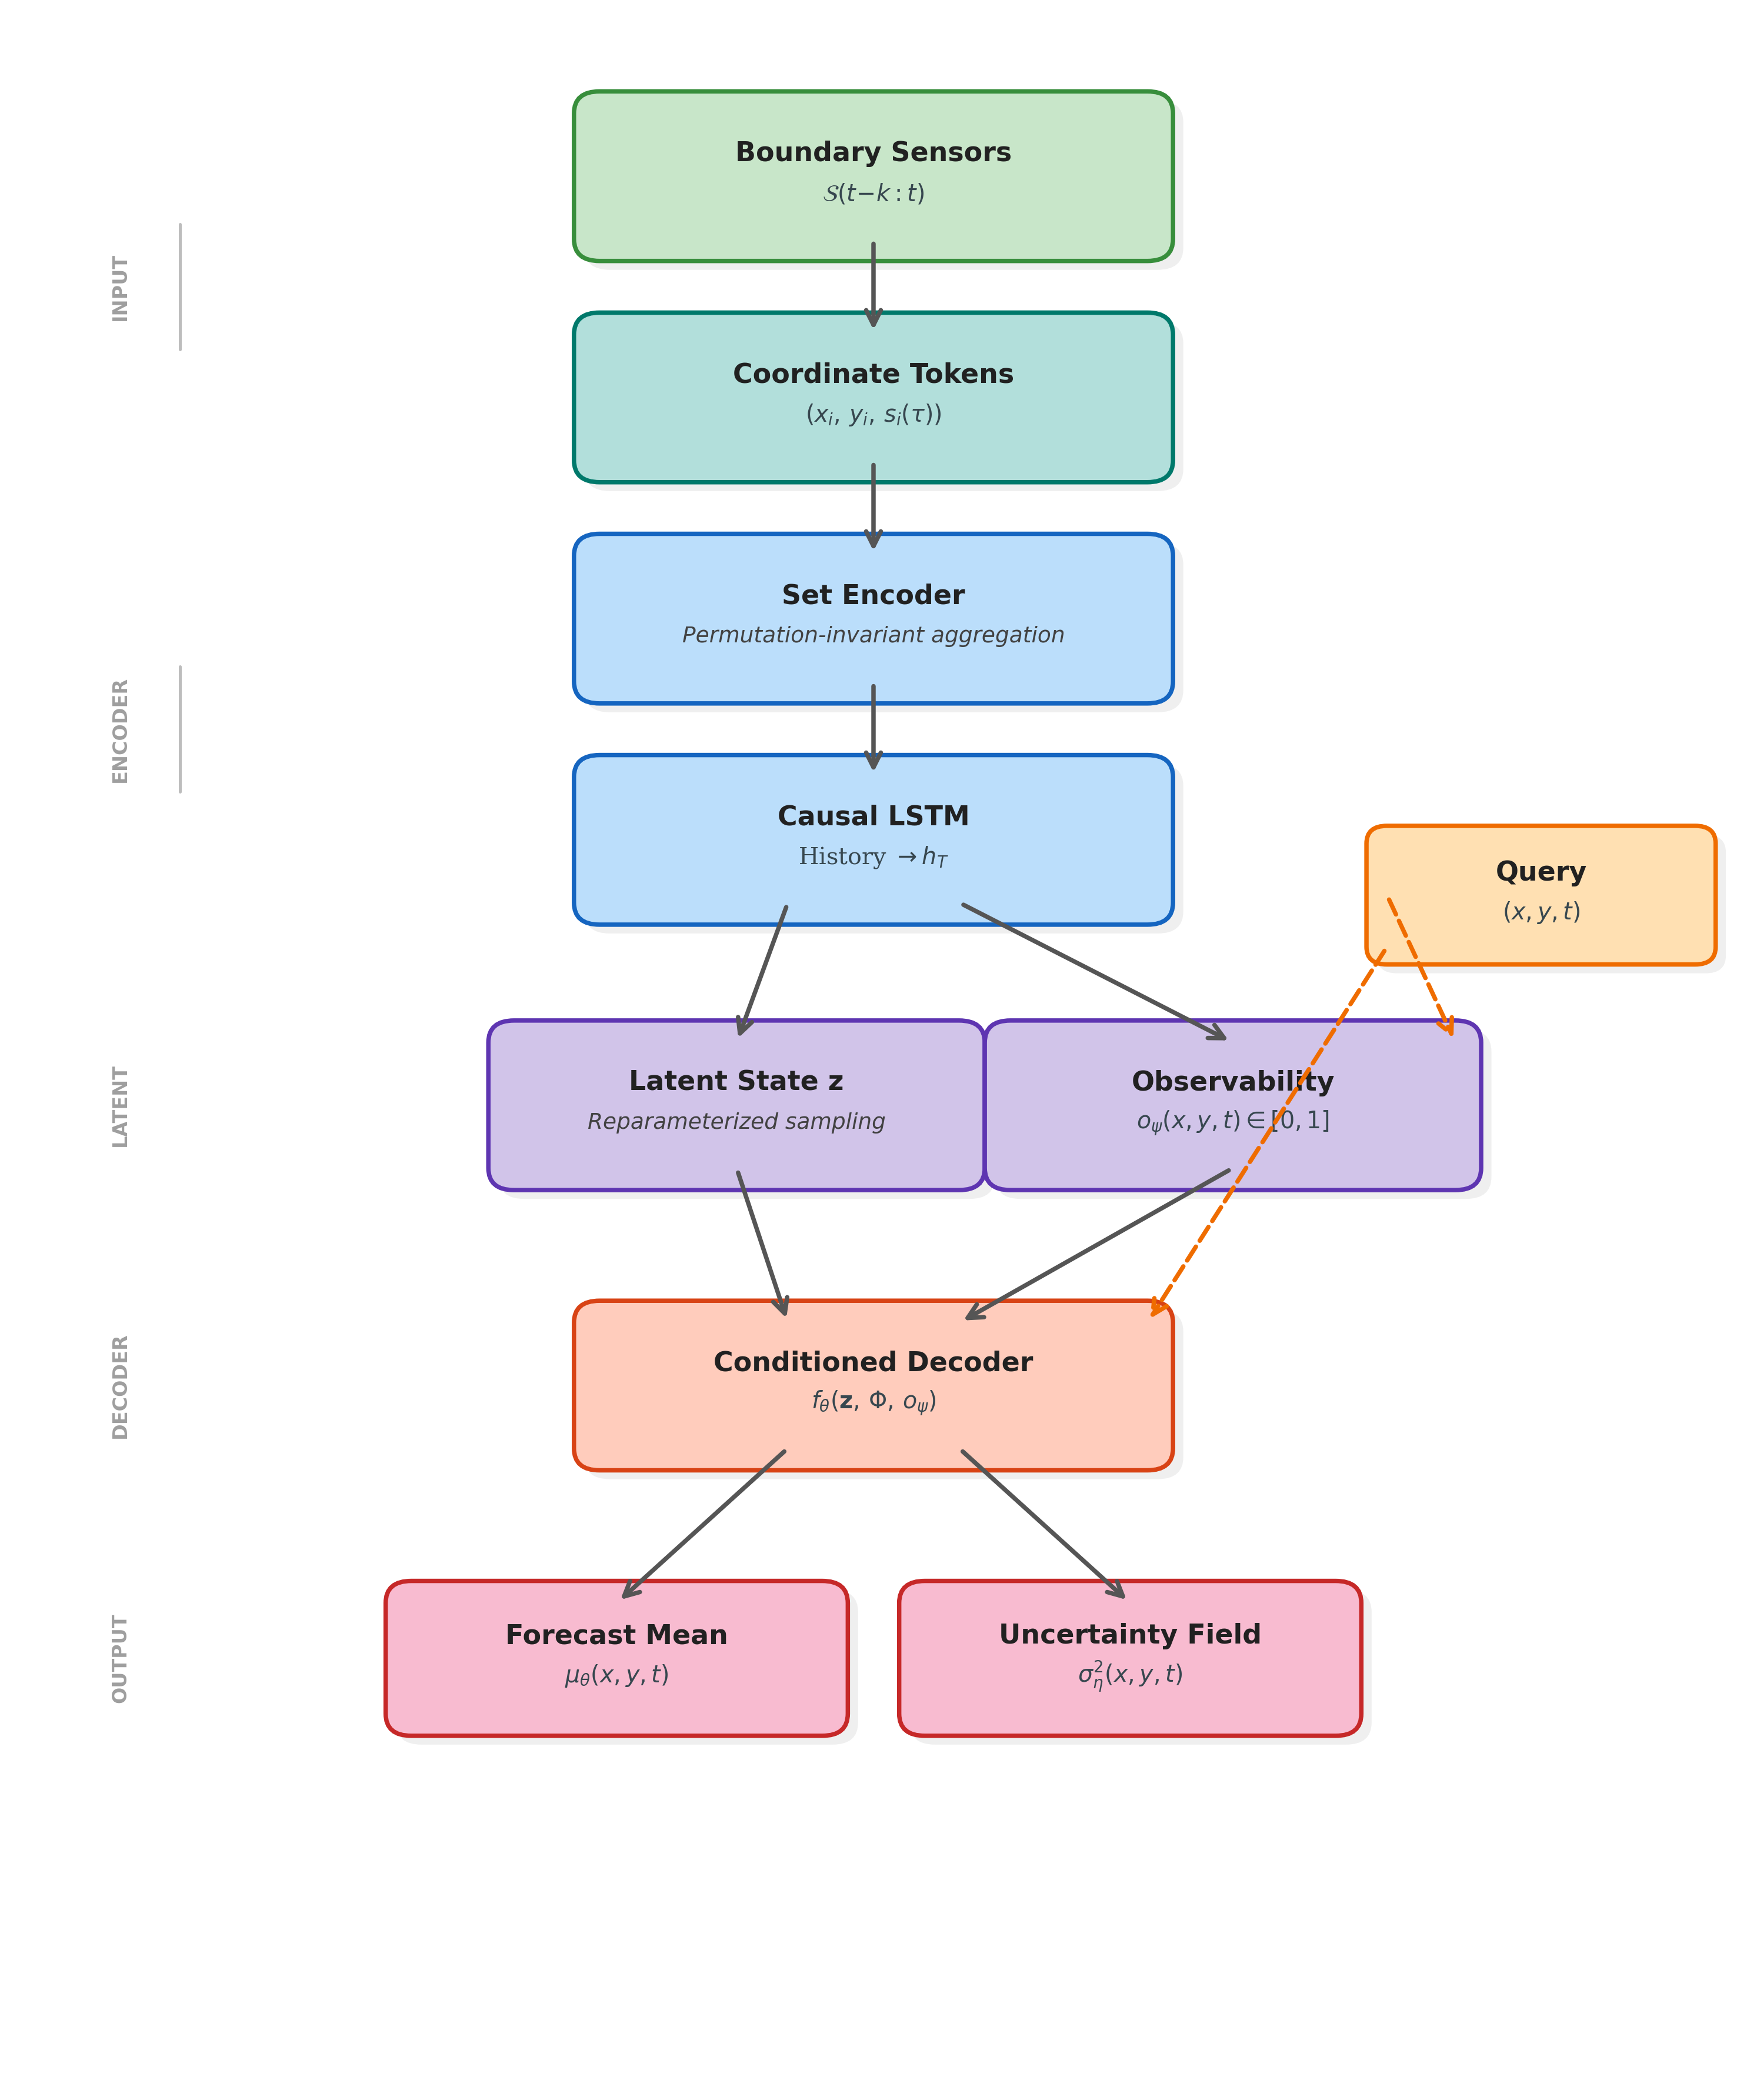
\includegraphics[height=0.78\textheight,keepaspectratio]{../docs/figures/ovcno_architecture.png}
\end{frame}

\begin{frame}{Năm thành phần chính}
  \small
  \begin{enumerate}\itemsep4pt
    \item \textbf{Sensor-geometry encoder:} $e_k(t) = \mathrm{MLP}_s(x_k, y_k, s_k(t))$
    \par\hspace{1em}\textcolor{gray}{Mỗi cảm biến là coordinate-valued token; vị trí mang thông tin riêng.}

    \item \textbf{DeepSets aggregation:} $r_t = \mathrm{MLP}_{\text{pool}}\bigl(\tfrac{1}{K}\sum_k e_k(t)\bigr)$
    \par\hspace{1em}\textcolor{gray}{Permutation-invariant, hỗ trợ $K$ biến đổi.}

    \item \textbf{Causal LSTM:} $h_T = \mathrm{LSTM}(r_0, \ldots, r_T)$
    \par\hspace{1em}\textcolor{gray}{Strict causality theo cấu trúc.}

    \item \textbf{Variational latent + observability proxy:}
    \[
      z \sim \mathcal{N}(\mu_z, \mathrm{diag}(\sigma_z^2)), \quad
      o_\psi(x,y,t) = \sigma\bigl(g_\psi(h_T, x, y, t, d_s)\bigr) \in [0,1]
    \]
    \par\hspace{1em}\textcolor{gray}{$o_\psi$ là \alert{learned proxy}, không phải observability rank theo control theory.}

    \item \textbf{Observability-conditioned decoder:}
    \[
      (\mu_\eta, \log \sigma_\eta^2) = f_\theta\bigl(z, \phi(x,y,t), o_\psi(x,y,t)\bigr)
    \]
    \par\hspace{1em}\textcolor{gray}{Output Gaussian; train với NLL + $\beta$ KL ($\beta = 0.01$).}
  \end{enumerate}
\end{frame}

\begin{frame}{Đánh giá toàn diện}
  \small
  \begin{tabular}{@{}l p{8cm}@{}}
    \toprule
    \textbf{Loại metric} & \textbf{Đo} \\
    \midrule
    Point & RMSE, MAE, Rel-$L_2$ \\
    Probabilistic & NLL, CRPS \\
    Calibration & Coverage @ 95\%, Average interval width \\
    Reliability & Spearman $\rho(|\varepsilon|, \hat{\sigma})$ \\
    Sanity & Spatial std ratio (chống mean collapse) \\
    & Partial corr (kiểm soát distance) \\
    & MAE monotonic theo $\hat\sigma$ quintile \\
    Horizon-conditioned & Per-lead-time +1h, +3h, +6h, +12h, +24h \\
    Real-station OSSE & Real/Equispaced/Random tại $K{=}12$ \\
    Missing-sensor robustness & Dropout 100/75/50\% \\
    \bottomrule
  \end{tabular}
\end{frame}

% ════════════════════════════════════════════════════════════════
\section{Kết quả thực nghiệm}
% ════════════════════════════════════════════════════════════════

\begin{frame}{Kết quả 1 --- PDEBench 2D SWE (clean benchmark)}
  \small \centering
  \begin{tabular}{@{}l c c c c c@{}}
    \toprule
    \textbf{Model} & \textbf{Input regime} & \textbf{Rel-$L_2$} & \textbf{RMSE} & \textbf{NLL} & \textbf{Cov@95} \\
    \midrule
    U-Net (PDEBench) & Full state & $\sim$12.80\% & --- & --- & --- \\
    FNO-2D (PDEBench) & Full state & 5.13\% & --- & --- & --- \\
    \midrule
    Det. Causal Op. & 16 boundary & 4.46\% & 0.0125 & --- & --- \\
    VCO & 16 boundary & 4.42\% & 0.0121 & $-3.12$ & 94.8\% \\
    \alert{OVCNO (ours)} & \alert{16 boundary} & \alert{4.38\%} & \alert{0.0118} & \alert{$-3.25$} & \alert{95.2\%} \\
    \bottomrule
  \end{tabular}

  \vspace{12pt}
  \begin{block}{Quan sát}
    Với chỉ \alert{0.1\% diện tích lưới}, mô hình của ta cạnh tranh với FNO dùng full-field input. Trên benchmark sạch này, ba causal sparse-boundary models cho kết quả gần như nhau --- benchmark không phân biệt được.
  \end{block}
\end{frame}

\begin{frame}{Kết quả 2 --- Copernicus SSH Vịnh Bắc Bộ (applied OSSE)}
  \small \centering
  \begin{tabular}{@{}l c c c c c c@{}}
    \toprule
    \textbf{Model} & \textbf{RMSE}$\downarrow$ & \textbf{NLL}$\downarrow$ & \textbf{CRPS}$\downarrow$ & \textbf{Avg.W} & \textbf{Cov@95} & \textbf{Corr}$_S$ \\
    \midrule
    Optimal Interp. & 0.114 & --- & --- & --- & --- & --- \\
    Persistence & 0.082 & --- & --- & --- & --- & --- \\
    Det. Causal Op. & 0.068 & --- & --- & --- & --- & --- \\
    VCO & 0.077 & $-1.92$ & 0.043 & \alert{0.209} & \alert{79.7\%} & 0.446 \\
    \alert{OVCNO (ours)} & \alert{0.068} & \alert{$-2.39$} & \alert{0.036} & 0.287 & \alert{94.8\%} & \alert{0.523} \\
    \bottomrule
  \end{tabular}

  \vspace{10pt}
  \begin{block}{Đánh đổi quan trọng}
    OVCNO \alert{cải thiện calibration} (Cov 79.7\%$\to$94.8\%, NLL $-1.92 \to -2.39$) nhưng interval rộng hơn 37\%. Lợi ích chính: \alert{reliability}, không phải sharpness.
  \end{block}
\end{frame}

\begin{frame}{Horizon-conditioned --- OVCNO giữ coverage ổn định}
  \small \centering
  \begin{tabular}{@{}l c c c c@{}}
    \toprule
    \textbf{Lead} & \textbf{VCO Cov} & \textbf{OVCNO Cov} & \textbf{VCO NLL} & \textbf{OVCNO NLL} \\
    \midrule
    +1h & 84.3\% & \alert{93.2\%} & $-2.38$ & \alert{$-2.63$} \\
    +6h & 84.3\% & \alert{93.6\%} & $-2.34$ & \alert{$-2.59$} \\
    +12h & 83.3\% & \alert{94.2\%} & $-2.22$ & \alert{$-2.49$} \\
    +24h & \alert{77.3\%} & \alert{94.7\%} & $-1.74$ & \alert{$-2.32$} \\
    \bottomrule
  \end{tabular}

  \vspace{8pt}
  \begin{block}{Phát hiện then chốt}
    Khi horizon dài hơn: \alert{VCO under-cover ngày càng nặng} (84\%$\to$77\%). OVCNO \alert{giữ coverage 93--95\%} bằng cách \alert{tự động phình interval}. Đây là claim mạnh nhất của paper.
  \end{block}
\end{frame}

\begin{frame}{Real-station OSSE --- bố trí cảm biến thật vs.\ tổng hợp}
  \begin{columns}
    \column{0.55\linewidth}
      \centering
      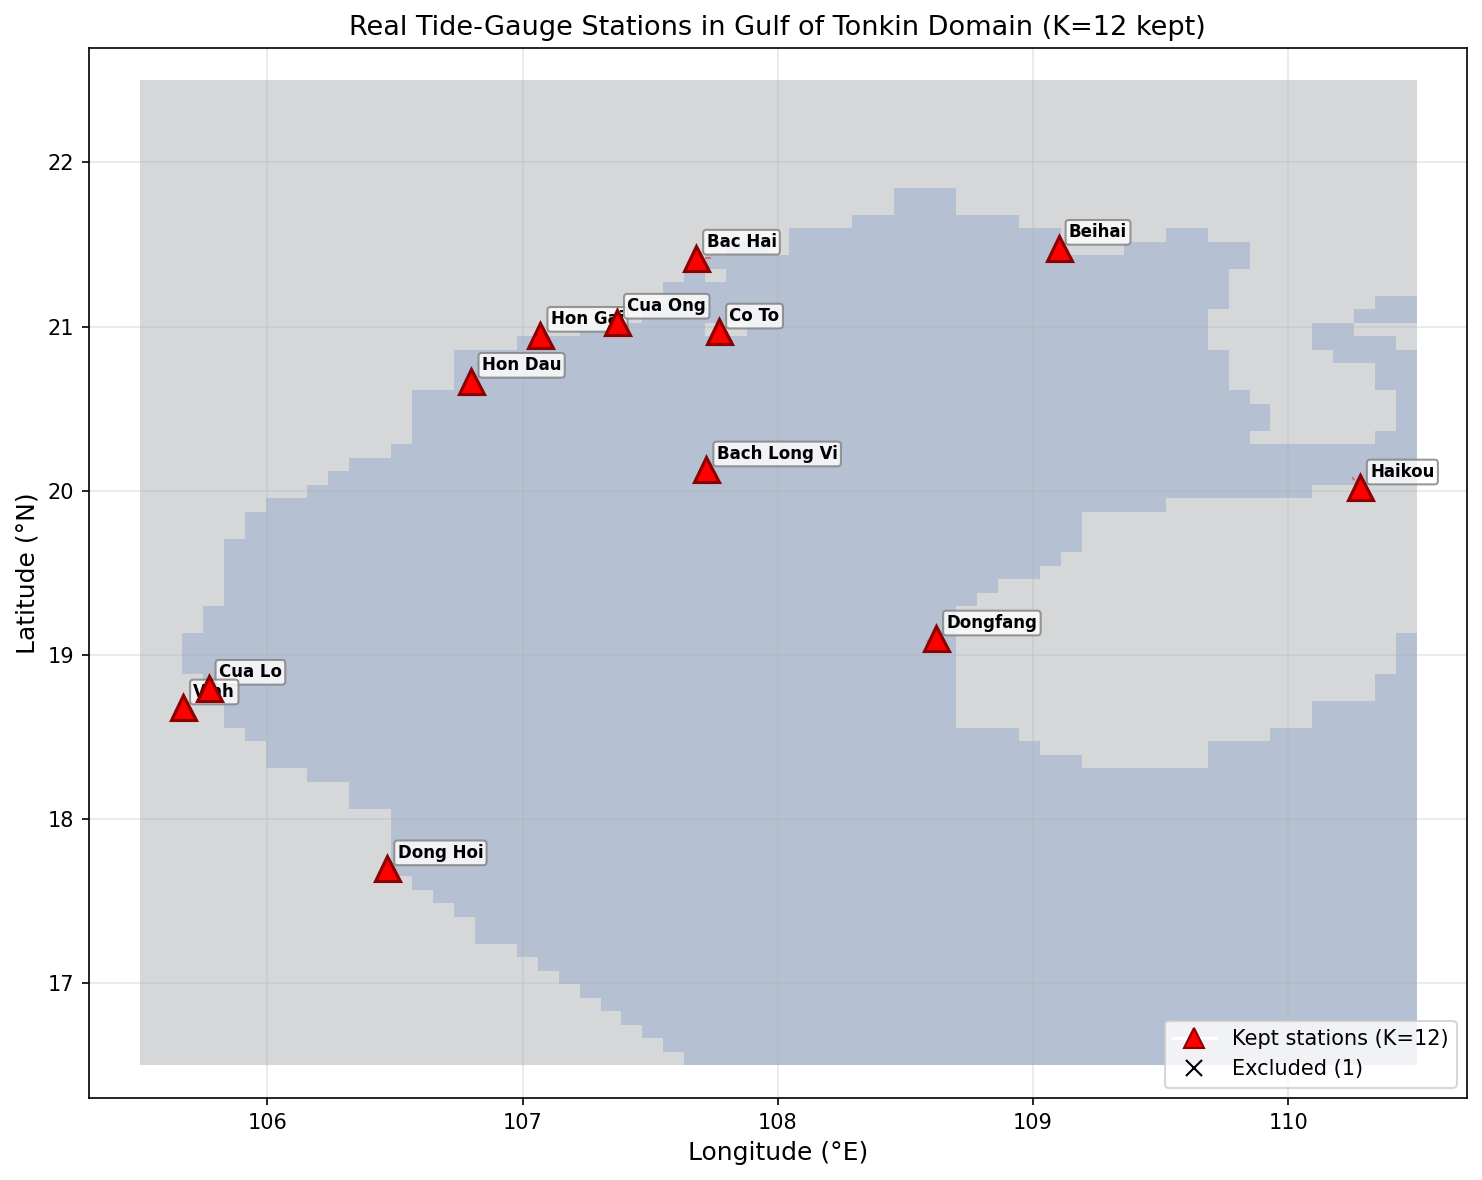
\includegraphics[width=\linewidth]{../docs/figures/station_map.png}

    \column{0.45\linewidth}
      \small
      \textbf{12 trạm thật} từ GLOSS/PSMSL/IOC trong Vịnh Bắc Bộ, so với:
      \begin{itemize}\itemsep1pt
        \item Equispaced-K12 (dàn đều)
        \item Random-K12 (lấy ngẫu nhiên)
      \end{itemize}

      \vspace{6pt}
      \textbf{Phát hiện:}
      \begin{itemize}\itemsep1pt
        \item Tại $K{=}12$, RMSE \alert{không khác biệt rõ rệt}.
        \item Training-seed variance \alert{lớn gấp $\sim$33$\times$} layout variance.
        \item Real-K12 vượt trội về \alert{robustness dropout} (Avg.W tăng chỉ 0.8\% vs 5.7\% cho Equispaced).
      \end{itemize}
  \end{columns}
\end{frame}

\begin{frame}{Học từ negative result --- HYCOM cross-product}
  \small
  \textbf{Initial:} OVCNO trên HYCOM cho Corr$_S = 0.41$ $\Rightarrow$ "OVCNO generalizes".

  \vspace{6pt}
  \textbf{Diagnostic Phase:}
  \begin{itemize}\itemsep2pt
    \item Spatial prediction maps: mean predictor \alert{collapse về gần hằng số}.
    \item SpatialStdRatio drop 1.54 (Copernicus) $\to$ \alert{0.38 (HYCOM)}.
    \item 4 ablation variants $\Rightarrow$ khi fix mean, RMSE 0.045 nhưng \alert{Corr$_S \to 0$}.
    \item Round 2 decoupled architecture: StdRatio stuck $\in [0.29, 0.33]$ \alert{bất kể} architecture.
  \end{itemize}

  \vspace{6pt}
  \begin{alertblock}{Quyết định khoa học}
    Corr$_S = 0.41$ là \alert{artifact của mean collapse}, không phải genuine UQ.
    $\Rightarrow$ \textbf{Loại HYCOM khỏi paper main body}, lưu làm research journal.
  \end{alertblock}

  \vspace{4pt}
  \textcolor{gray}{\footnotesize Đây là điểm mạnh khoa học: thừa nhận negative result thay vì spin nó. Documented đầy đủ trong \texttt{hycom\_complete\_report.md} + \texttt{hycom\_v2\_experiments.md}.}
\end{frame}

\begin{frame}{Sanity checks --- 5 chẩn đoán chống artifact}
  \small \centering
  \begin{tabular}{@{}l c l@{}}
    \toprule
    \textbf{Diagnostic} & \textbf{Result} & \textbf{Interpretation} \\
    \midrule
    Spatial std ratio (pred/gt) & \alert{1.54} & Không có mean collapse \\
    Partial Corr$(|\varepsilon|, \hat\sigma \mid d_s)$ & \alert{0.564} & Không phải distance confound \\
    Good-sample Corr$_S$ & 0.272 & Không phải outlier driven \\
    Bad-sample Corr$_S$ & 0.290 & Đồng đều \\
    MAE theo $\hat\sigma$ quintile & $0.027 \to 0.117$ & \alert{Monotonic risk stratification} \\
    \bottomrule
  \end{tabular}

  \vspace{10pt}
  \begin{block}{Tại sao 5 chẩn đoán này quan trọng?}
    Để chứng minh OVCNO trên Copernicus \alert{KHÔNG} bị cùng artifact như HYCOM. Reviewer cẩn thận sẽ kiểm tra ngay --- ta proactively trả lời.
  \end{block}
\end{frame}

% ════════════════════════════════════════════════════════════════
\section{Phân tích định tính}
% ════════════════════════════════════════════════════════════════

\begin{frame}{Observability proxy phát hiện được vùng khó}
  \centering
  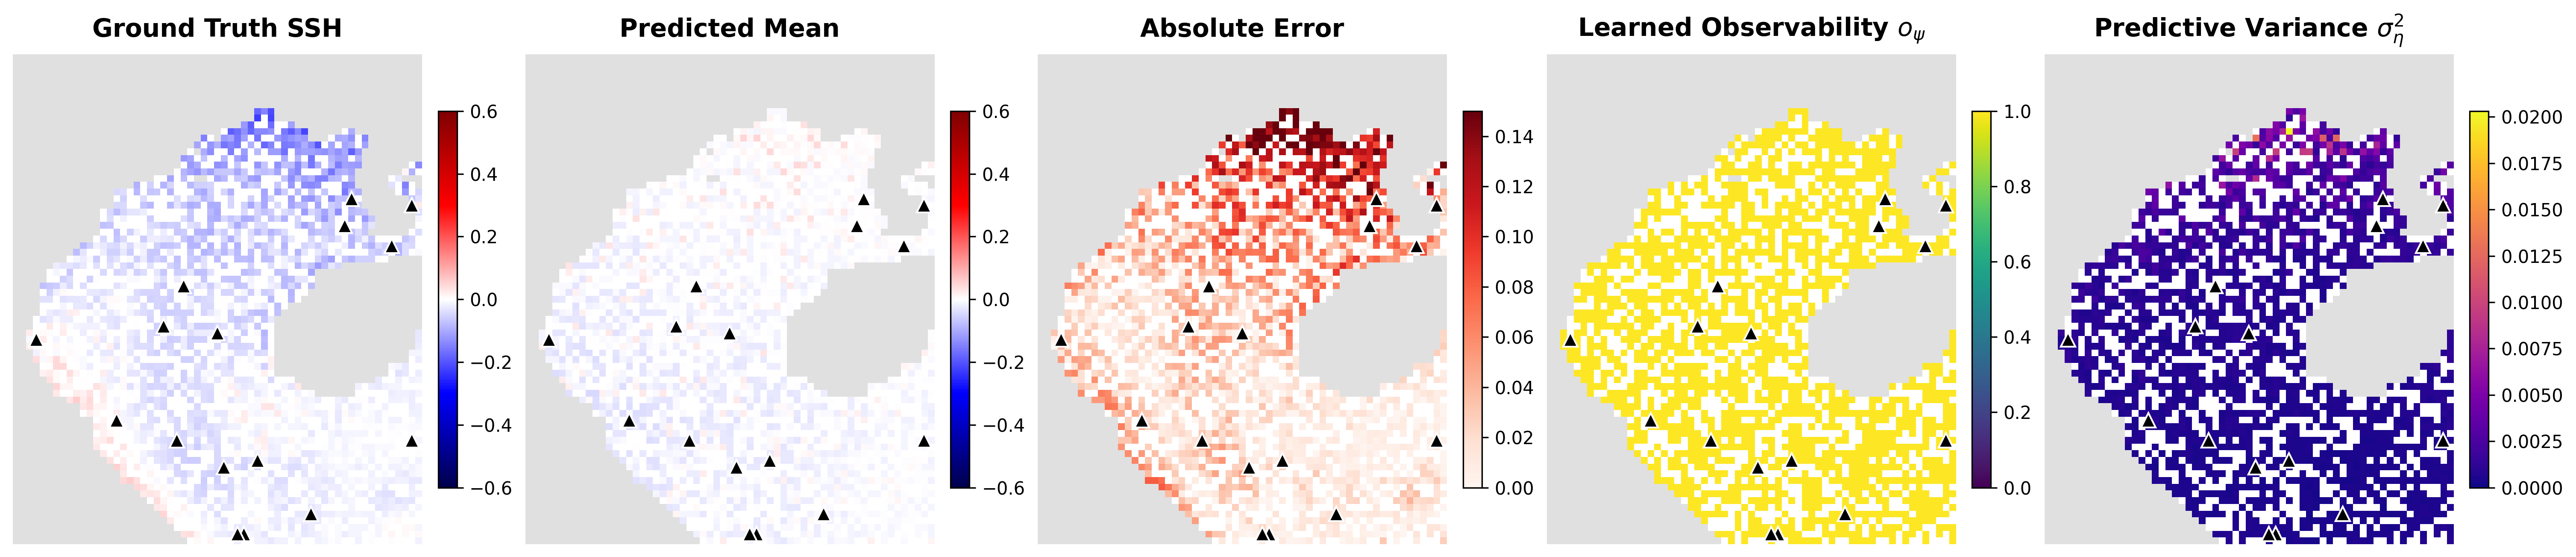
\includegraphics[width=0.96\linewidth]{../docs/figures/observability_maps.png}

  \vspace{4pt}
  \small \textcolor{gray}{Trái sang phải: SSH ground truth, predicted mean, $|error|$, learned $o_\psi$, $\hat\sigma$. Vùng $o_\psi$ cao $\to$ error thấp $\to$ $\hat\sigma$ thấp.}
\end{frame}

\begin{frame}{Bất định tăng dần theo khoảng cách tới cảm biến}
  \centering
  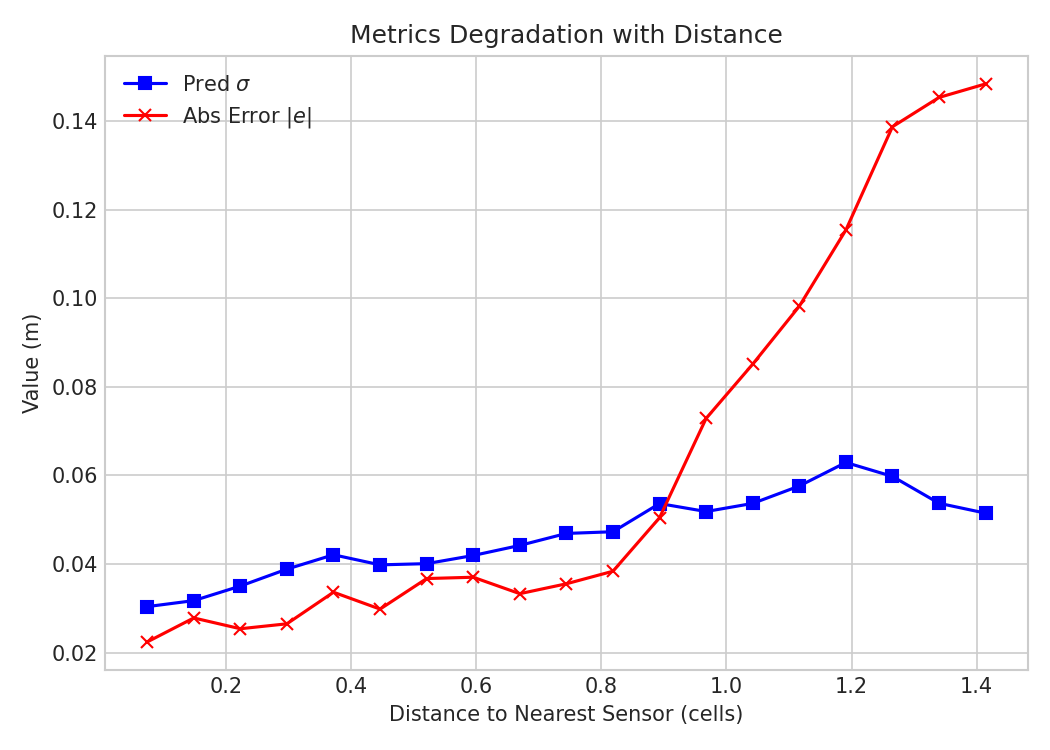
\includegraphics[width=0.55\linewidth]{../docs/figures/uncertainty_vs_distance.png}

  \vspace{6pt}
  \small
  Mô hình tự "học được" giới hạn thông tin: gần biên $\to \hat\sigma$ thấp; xa biên $\to \hat\sigma$ phình lên. \textbf{Cảnh báo thay vì cố gắng gượng ép}.
\end{frame}

% ════════════════════════════════════════════════════════════════
\section{Tổng kết}
% ════════════════════════════════════════════════════════════════

\begin{frame}{Đóng góp chính}
  \begin{block}{Bốn đóng góp}
    \begin{enumerate}\itemsep4pt
      \item \textbf{Problem formulation:} causal sparse-boundary-to-full-field as partially observable inverse forecasting.
      \item \textbf{OVCNO architecture:} sensor-geometry encoding + DeepSets + causal LSTM + variational latent + \alert{learned observability proxy}.
      \item \textbf{Empirical validation:} Copernicus Gulf of Tonkin OSSE --- Cov 79.7\%$\to$94.8\%, NLL $-1.92 \to -2.39$, Corr$_S$ 0.446$\to$0.523.
      \item \textbf{Real-station-geometry study:} layout topology ảnh hưởng \alert{robustness}, không phải nominal accuracy ở $K=12$.
    \end{enumerate}
  \end{block}
\end{frame}

\begin{frame}{Giới hạn (thẳng thắn thừa nhận trong paper §5)}
  \small
  \begin{enumerate}\itemsep3pt
    \item \alert{Validation $\ne$ test} --- 1 tháng dữ liệu, checkpoint selection cùng period.
    \item \textbf{Calibration-sharpness trade-off} --- interval rộng hơn VCO.
    \item \textbf{Level-1 OSSE} --- coordinate thật, value vẫn từ Copernicus.
    \item \textbf{Mean-variance coupling} --- gây mean collapse trên HYCOM.
    \item \textbf{Training-seed variance} > layout variance tại $K{=}12$.
    \item \textbf{Observability proxy moderate} --- Pearson $\approx$ 0.22.
  \end{enumerate}

  \vspace{6pt}
  \begin{block}{Tại sao thừa nhận?}
    Reviewer kỹ tính sẽ bắt ra. Thừa nhận chủ động $\to$ tăng credibility.
  \end{block}
\end{frame}

\begin{frame}{Hướng phát triển tiếp theo}
  \small
  \textbf{Ưu tiên cao (fix limitations 1--3):}
  \begin{itemize}\itemsep2pt
    \item Multi-month dataset với separate val/test periods.
    \item Conformal calibration để recover sharpness.
    \item Decoupled mean-variance architecture (mean head blind to $o_\psi$).
  \end{itemize}

  \vspace{6pt}
  \textbf{Mở rộng dài hạn:}
  \begin{itemize}\itemsep2pt
    \item Level-2 OSSE với real tide-gauge measurements (GLOSS, IOC).
    \item Cross-product robustness study (CMEMS + HYCOM + NOAA CBOFS).
    \item Matched-seed ablations + sensor-placement sweep $K \in \{8,16,24,32\}$.
    \item Explicit supervision của observability proxy (control-theoretic Gramian).
    \item Multi-day autoregressive rollouts + multi-variable (SSH + currents + temperature).
  \end{itemize}
\end{frame}

\begin{frame}[plain]
  \centering
  \vspace{1.5cm}
  {\Huge \textbf{Cảm ơn thầy/cô đã lắng nghe}}\\[14pt]
  {\Large Sẵn sàng trả lời câu hỏi}\\[28pt]
  {\large Vũ Hùng Anh --- PTIT}\\[6pt]
  {\small \texttt{vuhunganh0301@gmail.com}}\\[4pt]
  {\small Repo: \texttt{github.com/scalliontor/Sparse\_sensor\_tidal}}\\[20pt]
  
\includegraphics[height=1.5cm]{Logo_PTIT_University.png}
\end{frame}

% ════════════════════════════════════════════════════════════════
\appendix
\section*{Backup}
% ════════════════════════════════════════════════════════════════

\begin{frame}{Backup --- Reproducibility config (Copernicus OSSE)}
  \small \centering
  \begin{tabular}{@{}l l@{}}
    \toprule
    \textbf{Parameter} & \textbf{Value} \\
    \midrule
    Dataset & Copernicus CMEMS SSH (Vịnh Bắc Bộ, Jan 2024) \\
    Domain & $105.5^\circ$E--$110.5^\circ$E, $16.5^\circ$N--$22.5^\circ$N \\
    Grid & $73 \times 61$ (ocean points $\approx 2{,}520$) \\
    Temporal resolution & 1 hour \\
    Input history & 24 steps (24 h) \\
    Forecast horizon & Mixed 1--24 h \\
    Train / val & 600 / 144 timesteps (chronological) \\
    Sensors (main) & 16 equispaced; 12 real-station (OSSE) \\
    \midrule
    Optimizer & AdamW, lr $10^{-3}$, batch 4, 100 epochs \\
    Latent / LSTM / Decoder dim & 256 / 256 / 256 \\
    Fourier feature frequencies & 64 \\
    KL coefficient $\beta$ & 0.01 \\
    MC samples at inference & 50 \\
    Hardware & NVIDIA L40S (48 GB) \\
    \bottomrule
  \end{tabular}
\end{frame}

\begin{frame}{Backup --- Robustness curve}
  \centering
  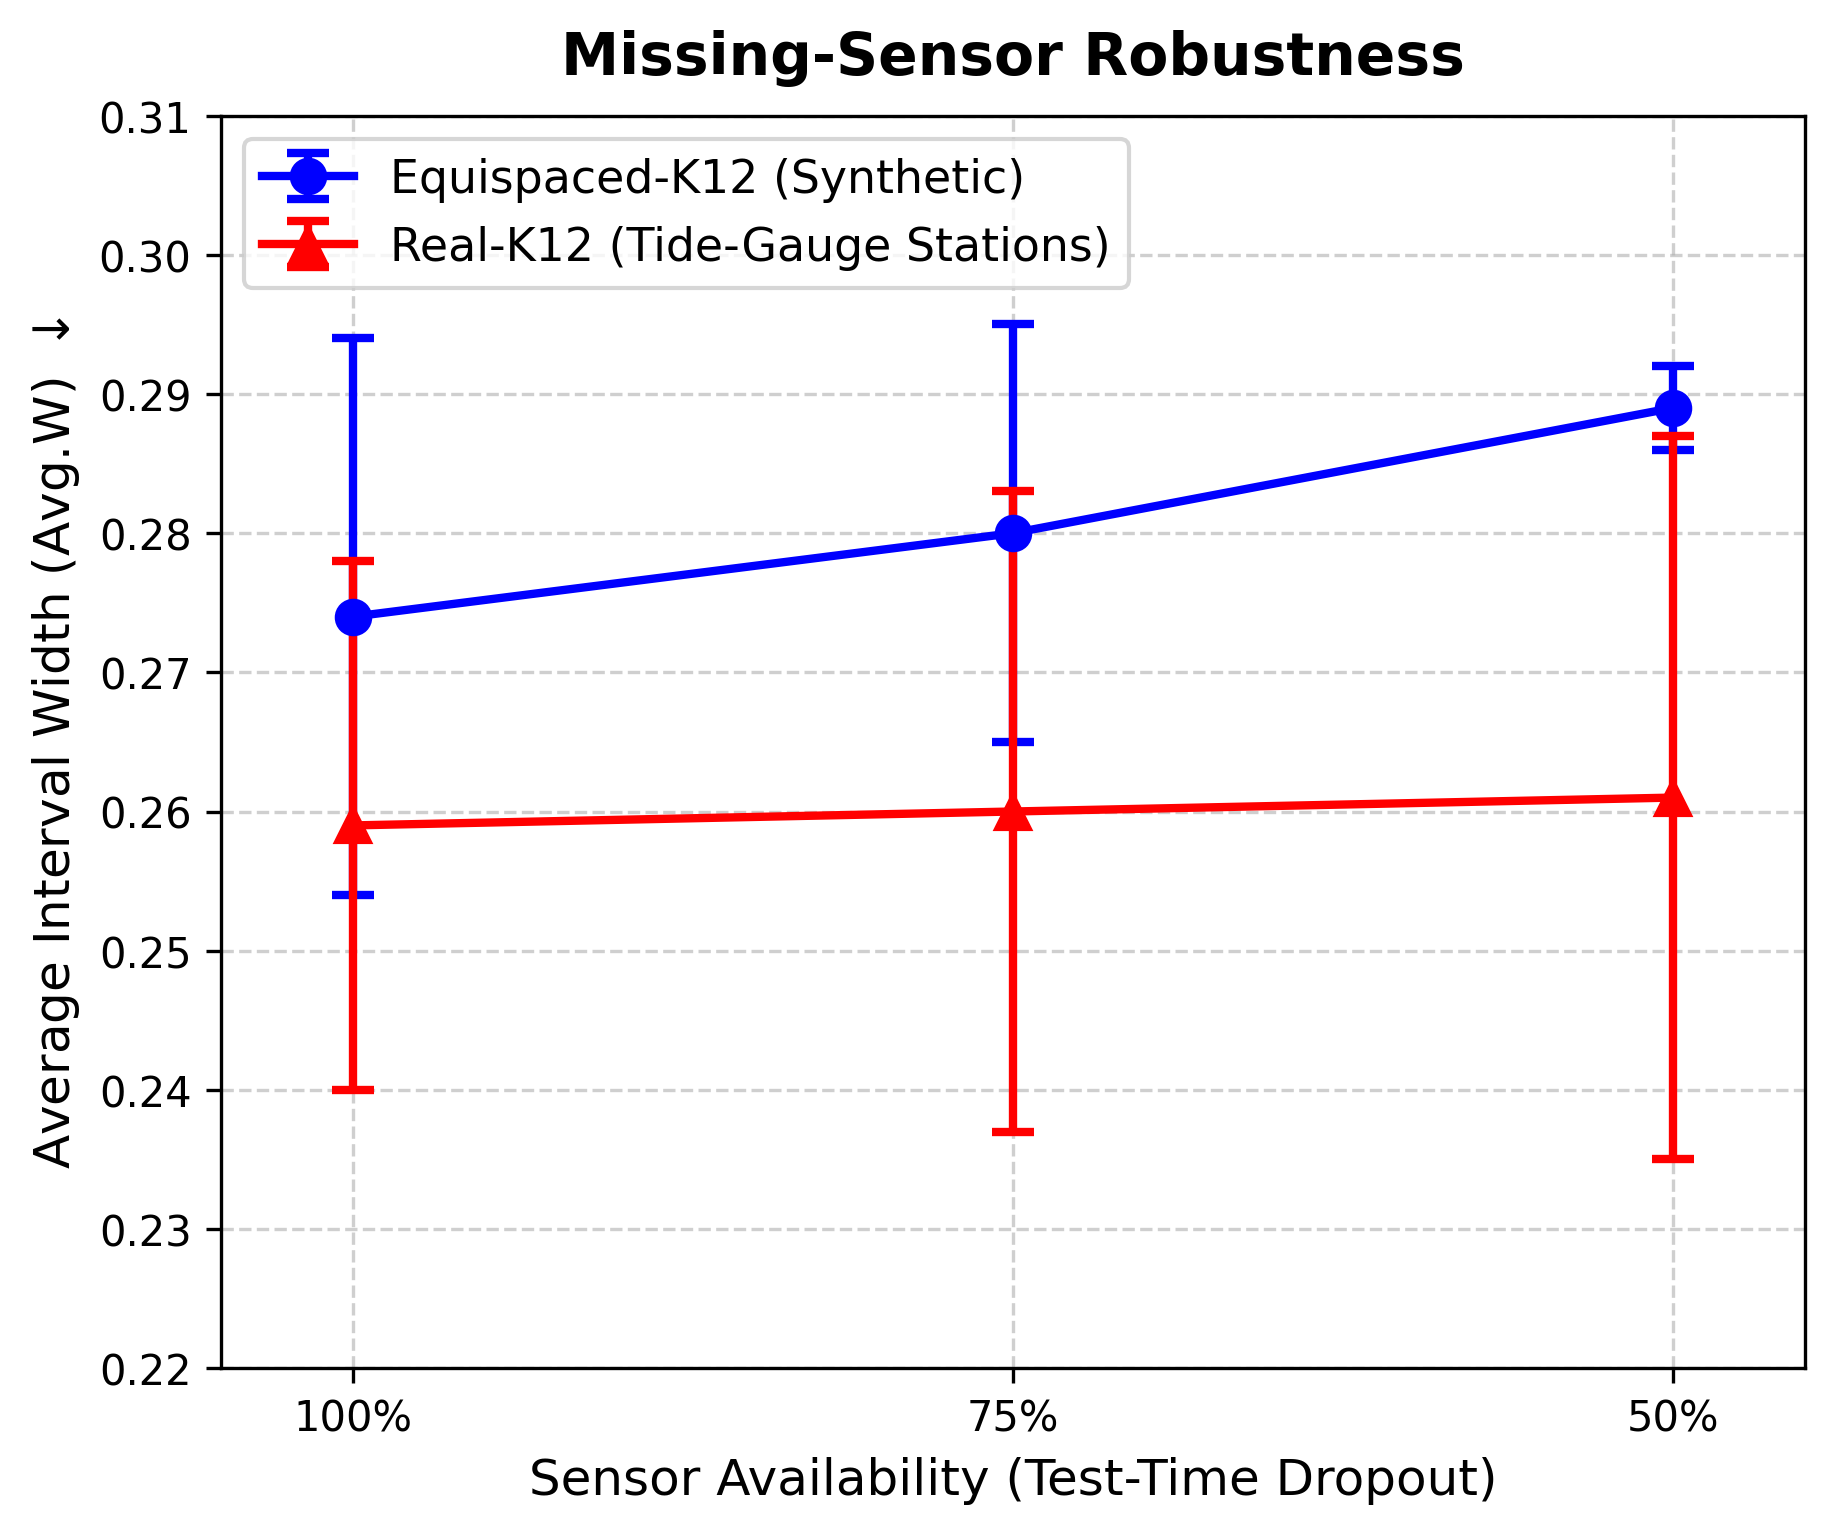
\includegraphics[height=0.7\textheight,keepaspectratio]{../docs/figures/robustness_curve.png}

  \vspace{2pt}
  {\small Real-K12 (đường liền): Avg.W gần như không đổi khi dropout 50\%; Equispaced-K12 tăng đều.}
\end{frame}

\begin{frame}{Backup --- Variance structure (layout vs.\ training seeds)}
  \centering
  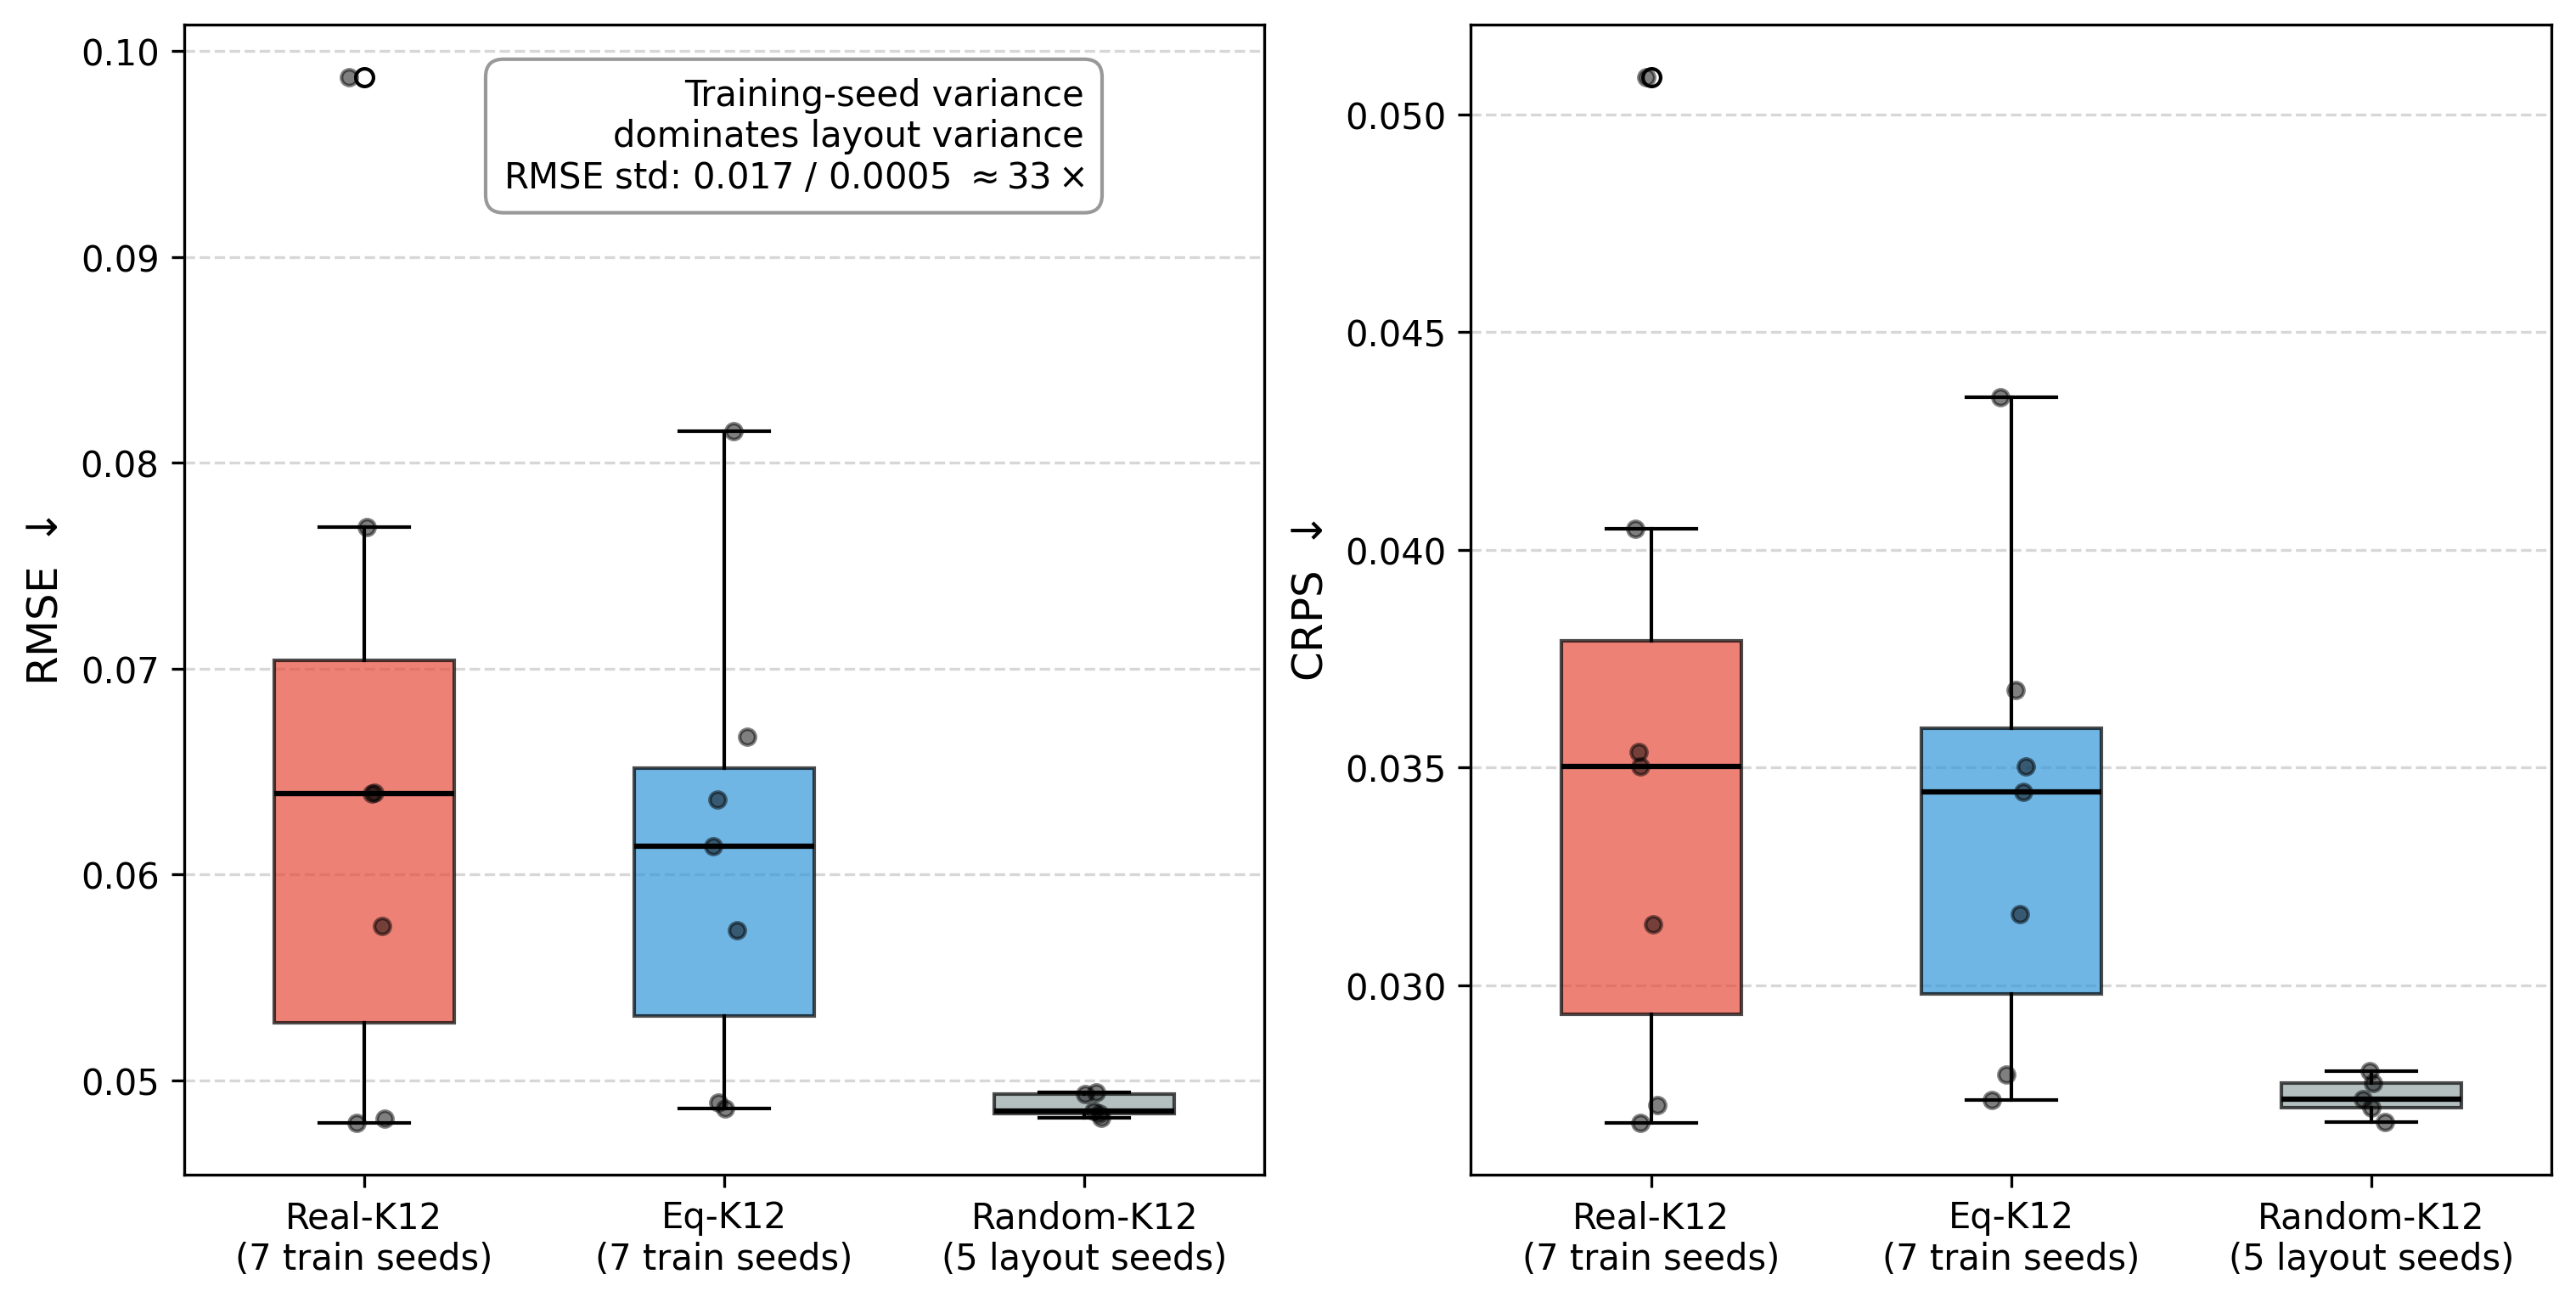
\includegraphics[height=0.7\textheight,keepaspectratio]{../docs/figures/topology_variance.png}

  \vspace{2pt}
  {\small Training-seed scatter \alert{lớn gấp $\sim$33$\times$} layout scatter.}
\end{frame}

\begin{frame}{Backup --- Forecast trajectories tại 3 điểm}
  \centering
  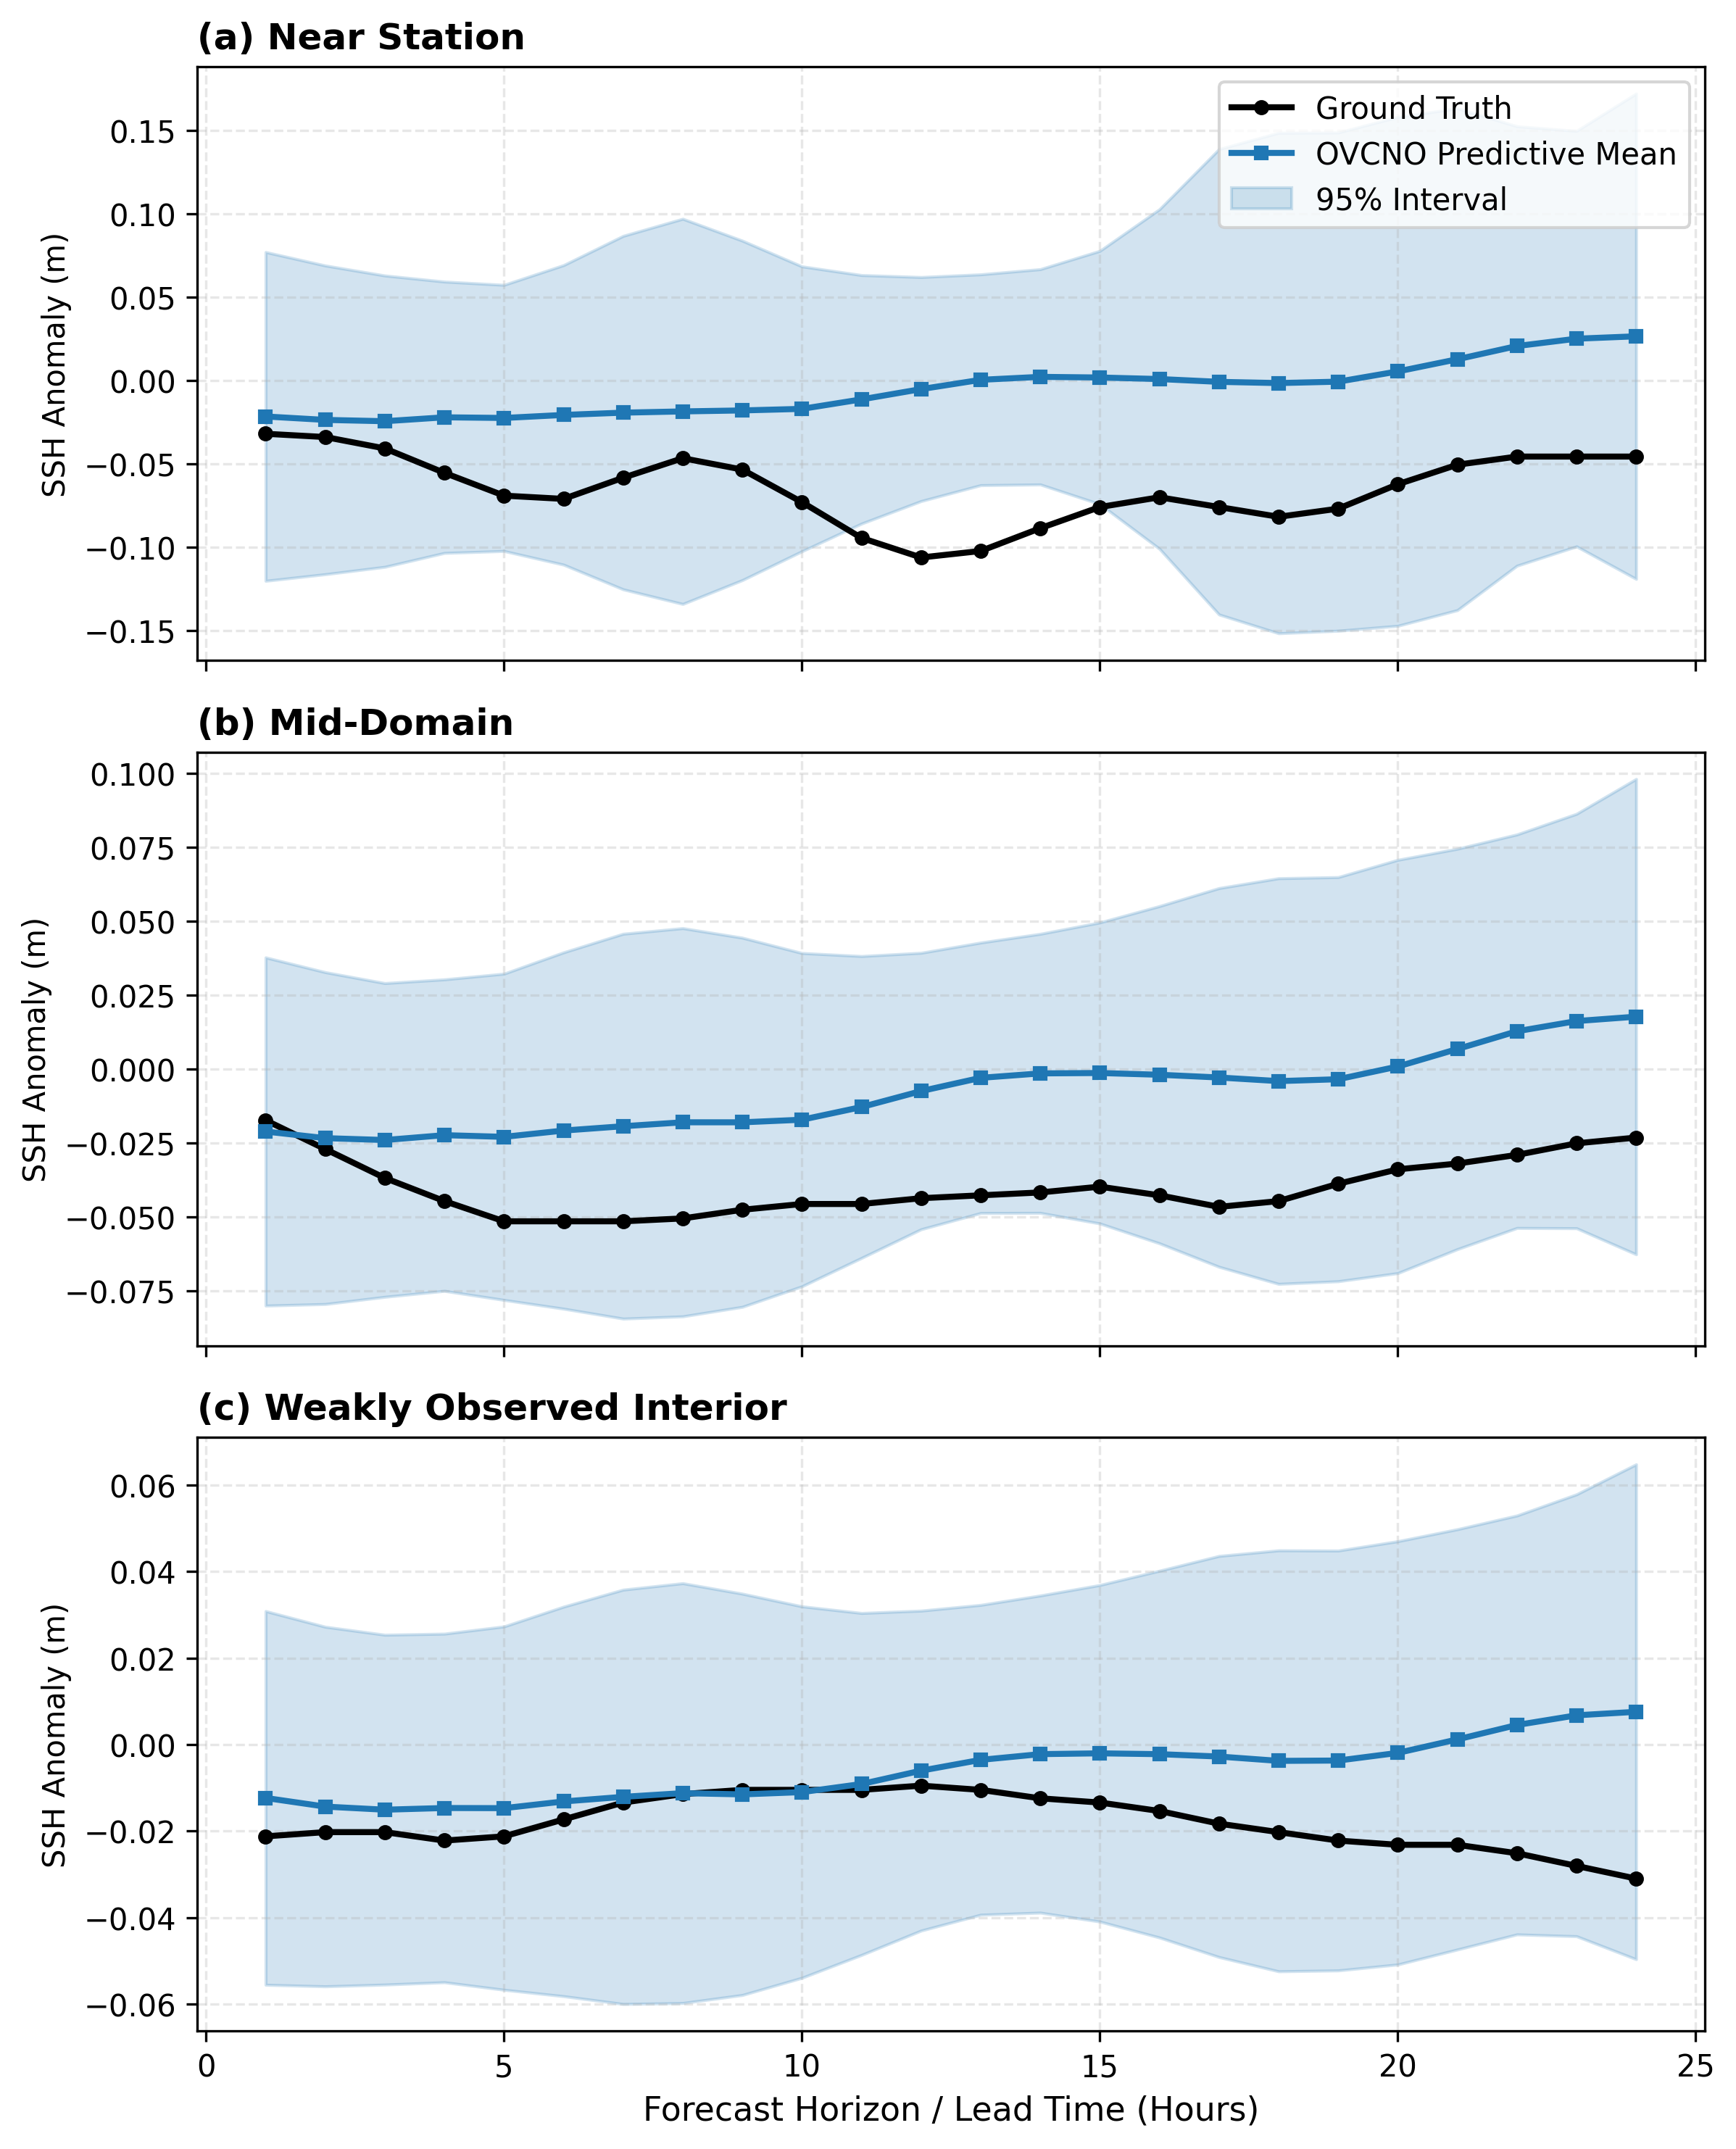
\includegraphics[height=0.7\textheight,keepaspectratio]{../docs/figures/forecast_trajectories.png}

  \vspace{2pt}
  {\small Quỹ đạo dự báo 1--24 h tại 3 điểm đại diện cho 3 chế độ observability khác nhau.}
\end{frame}

\end{document}
